\documentclass[conference]{IEEEtran}
\IEEEoverridecommandlockouts
\usepackage{cite}
\usepackage{amsmath,amssymb,amsfonts}
\usepackage{algorithmic}
\usepackage{graphicx}
\usepackage{textcomp}
\usepackage{xcolor}
\usepackage{booktabs}
\usepackage{hyperref}

\def\BibTeX{{\rm B\kern-.05em{\sc i\kern-.025em b}\kern-.08em
    T\kern-.1667em\lower.7ex\hbox{E}\kern-.125emX}}

\begin{document}

\title{Predicting Customer Response to Marketing Campaigns Using Supervised Machine Learning\\
% {\footnotesize \textsuperscript{*}Note: Sub-titles are not captured in Xplore and should not be used}
}

\author{\IEEEauthorblockN{1\textsuperscript{st} Given Name Surname}
\IEEEauthorblockA{\textit{dept. name of organization (of Aff.)} \\
\textit{name of organization (of Aff.)}\\
City, Country \\
email address or ORCID}
}

\maketitle

\begin{abstract}
% [WRITING GUIDANCE]
% The abstract should be approximately 150-250 words.
% 1. Start with a sentence about the broad business context (marketing campaigns, data mining).
% 2. State the specific problem: predicting customer response.
% 3. Briefly mention the methodology used (CRISP-DM, supervised learning algorithms).
% 4. State the most important finding (e.g., best performing model and its F1-score/ROC-AUC).
% 5. Conclude with the business implication of this result.

% Write your abstract here...

\end{abstract}


\begin{IEEEkeywords}
Data Mining, Supervised Learning, Customer Segmentation, Marketing Response, CRISP-DM
\end{IEEEkeywords}

\section{Introduction}
% [WRITING GUIDANCE]
% Target length: 0.75 - 1 column.
% Explain the business problem here.
% Describe why customer response prediction is important for marketing efficiency.
% State the primary research question.
% Briefly outline the structure of the rest of the paper.

% Write your introduction here...

\section{Related Work}
% [WRITING GUIDANCE]
% Target length: 0.5 - 0.75 column.
% Discuss prior literature on customer segmentation and campaign prediction.
% Mention approaches that used unsupervised clustering vs. supervised classification.
% Cite at least 3-5 relevant papers using \cite{placeholder1}, \cite{placeholder2}.

% Write your literature review here...

\section{Dataset and Exploratory Data Analysis}
% [WRITING GUIDANCE]
% Target length: 1 column.
% Describe the source of the data and its original features.
% Discuss the target variable (Response) and its class imbalance.

% Insert Figure 1 here. (Dataset Overview / Missing Values)
\begin{figure}[htbp]
\centerline{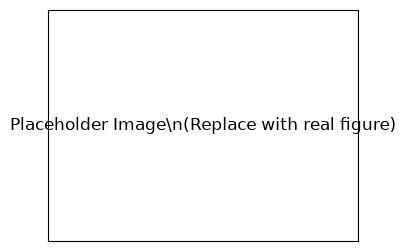
\includegraphics[width=\columnwidth]{figures/placeholder.png}}
\caption{Dataset Overview (Replace with actual missing values or descriptive plot).}
\label{fig:dataset_overview}
\end{figure}

% Insert Figure 2 here. (Target Distribution)
\begin{figure}[htbp]
\centerline{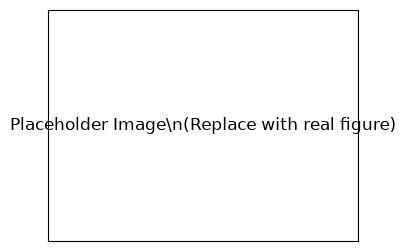
\includegraphics[width=0.7\columnwidth]{figures/placeholder.png}}
\caption{Target Distribution highlighting class imbalance.}
\label{fig:target_dist}
\end{figure}

% Insert Figure 3 here. (Correlation Matrix)
\begin{figure}[htbp]
\centerline{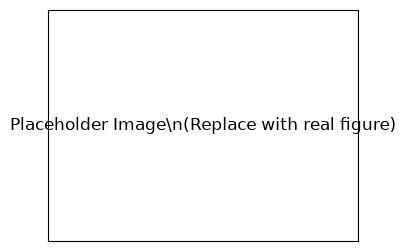
\includegraphics[width=\columnwidth]{figures/placeholder.png}}
\caption{Correlation Matrix of numeric features.}
\label{fig:correlation}
\end{figure}

% Insert Dataset Summary Table
\begin{table}[htbp]
\caption{Dataset Summary Statistics}
\begin{center}
\begin{tabular}{|l|c|c|}
\hline
\textbf{Feature} & \textbf{Data Type} & \textbf{Missing Values} \\
\hline
Income & Numeric & 24 \\
Education & Categorical & 0 \\
... & ... & ... \\
\hline
\end{tabular}
\label{tab:dataset_summary}
\end{center}
\end{table}

% Write your dataset description and EDA findings here...

\section{Methodology}
% [WRITING GUIDANCE]
% Target length: 1.5 - 2 columns.
% Discuss the CRISP-DM phases.

\subsection{Data Preprocessing and Feature Engineering}
% Summarize the preprocessing steps (imputation, outlier removal).
% Discuss the creation of composite business metrics (Customer_Value_Score, etc.).

% Insert Feature Engineering Summary Table
\begin{table}[htbp]
\caption{Feature Engineering Summary}
\begin{center}
\begin{tabular}{|l|p{5cm}|}
\hline
\textbf{New Feature} & \textbf{Derivation Logic} \\
\hline
Total\_Spending & Sum of all product category spending \\
Customer\_Value\_Score & Formula combining spending, acceptance, and recency \\
\hline
\end{tabular}
\label{tab:feature_eng}
\end{center}
\end{table}

\subsection{Feature Selection}
% Discuss methods used to reduce dimensionality (collinearity checks, RFE).

\subsection{Classification Algorithms}
% Describe the models compared: Decision Tree, Naive Bayes (GaussianNB), k-NN, Random Forest, XGBoost, etc.
% For Naive Bayes, state its conditional independence assumption.
% For k-NN, mention the distance metric and scaling requirement.

\subsection{Evaluation Metrics}
% Discuss why Accuracy is insufficient due to imbalance.
% Introduce F1-Score, ROC-AUC, and PR-AUC.

% Write your methodology details here...

\section{Experimental Results}
% [WRITING GUIDANCE]
% Target length: 1.5 - 2 columns.
% Present the quantitative results of the models.

\subsection{Hyperparameter Optimization}
% Discuss how GridSearchCV was used, specifically for k-NN (k=3,5,7,9,11) on the training set.

% Insert Hyperparameter Comparison Table
\begin{table}[htbp]
\caption{Hyperparameter Optimization Results (e.g., k-NN)}
\begin{center}
\begin{tabular}{|c|c|}
\hline
\textbf{Hyperparameter ($k$)} & \textbf{CV F1-Score} \\
\hline
3 & 0.xx \\
5 & 0.xx \\
7 & 0.xx \\
\hline
\end{tabular}
\label{tab:hyperparams}
\end{center}
\end{table}

\subsection{Model Comparison}
% Compare the final performance of all classifiers on the test set.

% Insert Final Evaluation Metrics Table
\begin{table}[htbp]
\caption{Final Evaluation Metrics on Test Set}
\begin{center}
\begin{tabular}{|l|c|c|c|c|}
\hline
\textbf{Model} & \textbf{Precision} & \textbf{Recall} & \textbf{F1-Score} & \textbf{ROC-AUC} \\
\hline
Decision Tree & 0.xx & 0.xx & 0.xx & 0.xx \\
Naive Bayes & 0.xx & 0.xx & 0.xx & 0.xx \\
k-NN & 0.xx & 0.xx & 0.xx & 0.xx \\
Random Forest & 0.xx & 0.xx & 0.xx & 0.xx \\
\hline
\end{tabular}
\label{tab:final_metrics}
\end{center}
\end{table}

% Insert Figure 4 here. (ROC Curves)
\begin{figure}[htbp]
\centerline{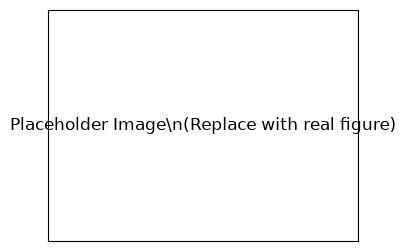
\includegraphics[width=\columnwidth]{figures/placeholder.png}}
\caption{ROC Curves for compared classifiers.}
\label{fig:roc}
\end{figure}

% Insert Figure 5 here. (Precision-Recall Curves)
\begin{figure}[htbp]
\centerline{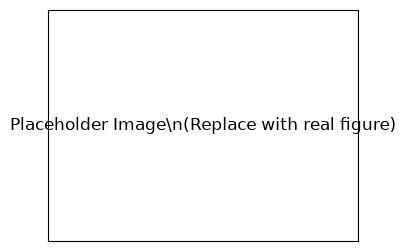
\includegraphics[width=\columnwidth]{figures/placeholder.png}}
\caption{Precision-Recall Curves for compared classifiers.}
\label{fig:pr}
\end{figure}

% Insert Figure 8 here. (Confusion Matrix)
\begin{figure}[htbp]
\centerline{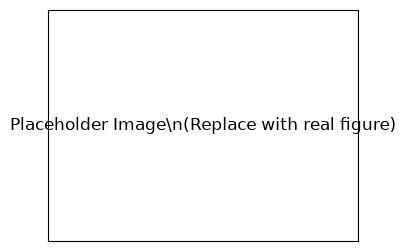
\includegraphics[width=0.8\columnwidth]{figures/placeholder.png}}
\caption{Confusion Matrix for the best performing model.}
\label{fig:conf_matrix}
\end{figure}

% Discuss why Random Forest (or the best model) outperformed Decision Tree or Naive Bayes.
% Write your results description here...

\section{Discussion and Interpretation}
% [WRITING GUIDANCE]
% Target length: 1 column.
% Interpret the results in a business context.
% Do NOT fabricate interpretations; base them on the SHAP or Feature Importance plots.

% Insert Figure 6 here. (Feature Importance)
\begin{figure}[htbp]
\centerline{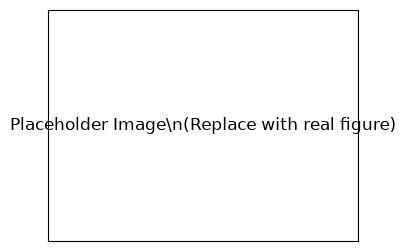
\includegraphics[width=\columnwidth]{figures/placeholder.png}}
\caption{Feature Importance Ranking of the best ensemble model.}
\label{fig:feat_imp}
\end{figure}

% Insert Figure 7 here. (SHAP Summary)
\begin{figure}[htbp]
\centerline{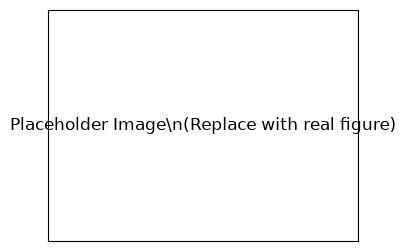
\includegraphics[width=\columnwidth]{figures/placeholder.png}}
\caption{SHAP Summary Plot illustrating directional impact of features.}
\label{fig:shap}
\end{figure}

% Insert Feature Importance Ranking Table
\begin{table}[htbp]
\caption{Top 5 Most Important Features}
\begin{center}
\begin{tabular}{|c|l|}
\hline
\textbf{Rank} & \textbf{Feature Name} \\
\hline
1 & Customer\_Value\_Score \\
2 & Campaign\_Acceptance\_Count \\
3 & Recency \\
4 & ... \\
5 & ... \\
\hline
\end{tabular}
\label{tab:feat_ranking}
\end{center}
\end{table}

% Discuss what these features mean for the marketing department.
% Write your discussion here...

\section{Conclusion and Future Work}
% [WRITING GUIDANCE]
% Target length: 0.5 column.
% Summarize the main achievements of the project.
% State the final business recommendation based on the model's predictions.
% Suggest future research directions (e.g., collecting more data, trying deep learning).

% Write your conclusion here...


\bibliographystyle{IEEEtran}
\bibliography{references}

\end{document}
